\documentclass[english,a4paper,12pt,oneside]{article}


%\includeonly{lab4}

%Drafting options
%uncomment for double spacing
%\doublespacing

% \usepackage{acronym}
\usepackage{times}
\usepackage{setspace} 
\usepackage{amsmath}    % need for subequations
\usepackage{graphicx}   % need for figures
%\usepackage{picture}
% \usepackage{wrapfig}
\usepackage{graphics}
 \graphicspath{{./}{../octave/}{../data/}}
 \usepackage{epstopdf}
\usepackage{color}
\usepackage{listings}
\lstset{language=C++,
	basicstyle=\ttfamily\footnotesize,
	breaklines=true,
%    basicstyle=\ttfamily,
    keywordstyle=\color{blue}\ttfamily,
    stringstyle=\color{red}\ttfamily,
    commentstyle=\color{green}\ttfamily,
%    morecomment=[l][\color{magenta}]{\#}
}
\usepackage{verbatim}   % useful for program listings
\usepackage{color}      % use if color is used in text
\usepackage{subfigure}  % use for side-by-side figures
\usepackage{varioref}
\usepackage{anysize}
\usepackage{natbib}
\usepackage{fancyhdr}
% \usepackage{units}
\usepackage{longtable}
%\usepackage{bbding}
%\usepackage{aeguill}
\usepackage[hyphens]{url}
\usepackage{hyperref}

\setlength{\parskip}{8pt plus 2pt minus 2pt}
\setlength{\parindent}{0pt}

\marginsize{2cm}{2cm}{2cm}{2cm}
\fancypagestyle{plain}{%
  \fancyhf{}%
  \renewcommand{\headrulewidth}{0pt}%
  \renewcommand{\footrulewidth}{0pt}%
}

\pagestyle{fancy}
%\renewcommand{\sectionmark}[1]{\markright{\thesection.\ #1}}

\renewcommand{\sectionmark}[1]{\markright{#1}{}}
\renewcommand{\subsectionmark}[1]{\markright{#1}{}}
\renewcommand{\subsubsectionmark}[1]{\markright{#1}{}}

%\renewcommand{\quote}[1]{\textit{\begin{quote}#1\end{quote}}}
\newcommand{\bold}[1]{\emph{\textbf{#1}}}

\newcommand{\varentry}[1]{{\guillemotleft}\emph{#1}{\guillemotright}}
\newcommand{\code}[1]{{\tt #1}}

\headheight 10mm


\rhead{15/11/2016}
\chead{}
\lhead{ICP3038 --- Computer Vision}
\rfoot{}
\cfoot{- \thepage  \,\,-}
\lfoot{}

\renewcommand{\headrulewidth}{0.4pt}
\renewcommand{\footrulewidth}{0.4pt} 



\begin{document}
% !TEX root = ./ICP3038_Lab_03.tex

\section*{Laboratory 4: How to compare 1D arrays}

%This is a typical script that you will be working with at each
%laboratory session. To work with these scripts efficiently, follow the
%guidelines below.
%\begin{enumerate}
%  \item The script is not a step-by-step tutorial. It introduces the
%    problem but it is your task to solve it.
%
%  \item If you get stuck, make sure that you read \emph{Help} section
%    at the end of the document.
%
%  \item If you still have problems, ask the lecturer, demonstrator or
%    fellow students for help.
%
%  \item Try to do as much work as possible in the class, where it is
%    easier to get help.
%    
%  \item If you need help when working at home, use the Blackboard
%    discussion board.
%    
%  \item Finish all assignments at least a week before the deadline. If you get
%    stuck, you will still have one week to ask for help.
%\end{enumerate}

The aims of today's lab are:
\begin{itemize}
	\item Use the STL vector class to store an array of \verb+float+ values;
	\item Use built-in functions to compute the min, max, and sum of the array;
%	\item Compute the histogram (with the number of bins as a parameter of the function);
	\item Compare two arrays using the Sum of Absolute Errors (SAE) and the normalised cross-correlation (NCC).
%	\item Compare two arrays using \verb+operator==+ and \verb+operator!=+.
\end{itemize}

Note, today you work using 1-D arrays. In Assignment~2, you have to do the same in 2-D with images.

\section*{Task 0: Using CMake}

Same as usual, we will use CMake to make our lives easier. 
%In the lecture, you saw yesterday that it can be extremely complicated to use the IDE to maintain the project files, etc. particularly if students use Windows, Mac, or Linux. 
%There is a ZIP file on Blackboard with 4 (almost) empty C++ source files. There is also a `CMakeLists.txt' file. 
%It is a good practice to organise your source code using directories, etc. Do not compile code in the same directory as your source code. It can get messy... 
%Extract the ZIP file, and set up the compilation environment using \verb+cmake+. 
%In the GUI, the source directory corresponds to the direction in which `CMakeLists.txt' is. 
%The binary directory is where the code will be compiled. Often, we call this directory `bin'. 
%Once the paths are set, press `Configure'. 
%The first time you run the configuration tool, you have to select a generator.
%If you want to use MSVC++ in the lab, make sure to use \emph{Visual Studio 14 2015 Win64}. 
%For Mac OS X, you may want to use the Xcode generator. 
%For Linux, you may choose Makefile. 
%Once the configuration step is over, press `Generate'. 
%The project files are now ready in the `bin' directory. 
%You can compile the code using the preferred IDE.

\section*{Task 1: Min/Max/Sum/Average/Variance/Standard deviation}

You have been given a ZIP file containing a small (incomplete class). 
For this task, you mostly have to modify \verb+MyVector.cpp+.
The methods you need to complete are:
\begin{enumerate}
 \item \verb+float getMinValue() const+ (see previos labs)
 \item \verb+float getMaxValue() const+ (see previos labs)
 \item \verb+float getSum() const+ (see previos labs)
 \item \verb+float getAverage() const+
 \item \verb+float getVariance() const+
 \item \verb+float getStandardDeviation() const+
\end{enumerate}

In the ZIP file, you also got 4 ASCII files:
\begin{itemize}
 \item \verb+y.mat+
 \item \verb+y_quadriple.mat+
 \item \verb+y_noise.mat+
 \item \verb+y_negative.mat+
\end{itemize}
They contain test data that you can use to assess your code. 
Figure~\ref{fig:test data} shows the content of the files. 
You can load each file in independent instances of the class \verb+MyVector+. 
\begin{figure}[htb]
\centering
\scalebox{0.75}{% Title: glps_renderer figure
% Creator: GL2PS 1.3.8, (C) 1999-2012 C. Geuzaine
% For: Octave
% CreationDate: Mon Nov 16 16:43:05 2015
\setlength{\unitlength}{1pt}
\begin{picture}(0,0)
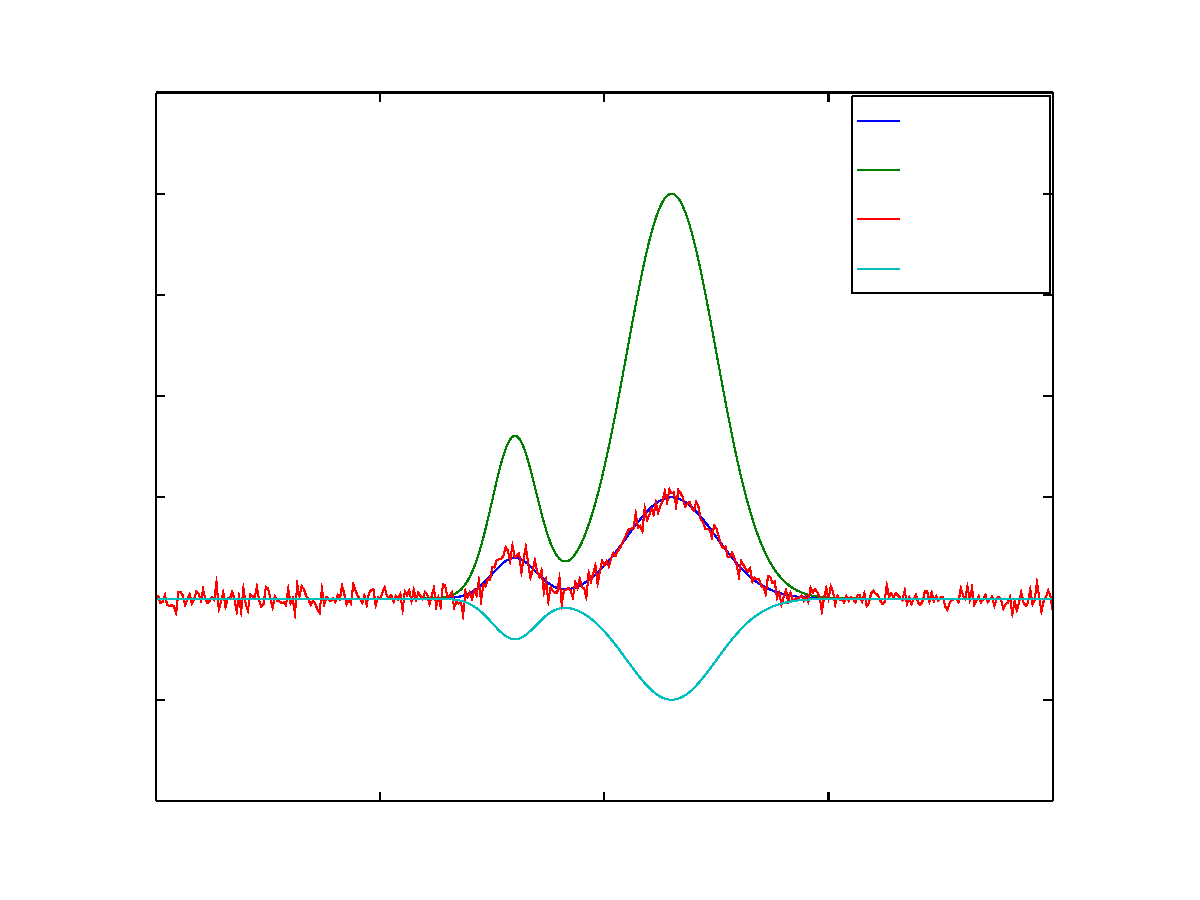
\includegraphics{curves-inc}
\end{picture}%
\begin{picture}(576,432)(0,0)
\fontsize{12}{0}
\selectfont\put(74.8799,42.519){\makebox(0,0)[t]{\textcolor[rgb]{0,0,0}{{-10}}}}
\fontsize{12}{0}
\selectfont\put(182.48,42.519){\makebox(0,0)[t]{\textcolor[rgb]{0,0,0}{{-5}}}}
\fontsize{12}{0}
\selectfont\put(290.08,42.519){\makebox(0,0)[t]{\textcolor[rgb]{0,0,0}{{0}}}}
\fontsize{12}{0}
\selectfont\put(397.68,42.519){\makebox(0,0)[t]{\textcolor[rgb]{0,0,0}{{5}}}}
\fontsize{12}{0}
\selectfont\put(505.28,42.519){\makebox(0,0)[t]{\textcolor[rgb]{0,0,0}{{10}}}}
\fontsize{12}{0}
\selectfont\put(69.8755,47.52){\makebox(0,0)[r]{\textcolor[rgb]{0,0,0}{{-10}}}}
\fontsize{12}{0}
\selectfont\put(69.8755,96.103){\makebox(0,0)[r]{\textcolor[rgb]{0,0,0}{{-5}}}}
\fontsize{12}{0}
\selectfont\put(69.8755,144.686){\makebox(0,0)[r]{\textcolor[rgb]{0,0,0}{{0}}}}
\fontsize{12}{0}
\selectfont\put(69.8755,193.269){\makebox(0,0)[r]{\textcolor[rgb]{0,0,0}{{5}}}}
\fontsize{12}{0}
\selectfont\put(69.8755,241.852){\makebox(0,0)[r]{\textcolor[rgb]{0,0,0}{{10}}}}
\fontsize{12}{0}
\selectfont\put(69.8755,290.434){\makebox(0,0)[r]{\textcolor[rgb]{0,0,0}{{15}}}}
\fontsize{12}{0}
\selectfont\put(69.8755,339.017){\makebox(0,0)[r]{\textcolor[rgb]{0,0,0}{{20}}}}
\fontsize{12}{0}
\selectfont\put(69.8755,387.6){\makebox(0,0)[r]{\textcolor[rgb]{0,0,0}{{25}}}}
\fontsize{12}{0}
\selectfont\put(290.08,397.6){\makebox(0,0)[b]{\textcolor[rgb]{0,0,0}{{Test data}}}}
\fontsize{12}{0}
\selectfont\put(434.47,374.002){\makebox(0,0)[l]{\textcolor[rgb]{0,0,0}{{$Y$}}}}
\fontsize{12}{0}
\selectfont\put(434.47,350.337){\makebox(0,0)[l]{\textcolor[rgb]{0,0,0}{{$Y_{quadriple}$}}}}
\fontsize{12}{0}
\selectfont\put(434.47,326.672){\makebox(0,0)[l]{\textcolor[rgb]{0,0,0}{{$Y_{noise}$}}}}
\fontsize{12}{0}
\selectfont\put(434.47,303.008){\makebox(0,0)[l]{\textcolor[rgb]{0,0,0}{{$Y_{negative}$}}}}
\end{picture}
}
 \caption{\label{fig:test data}Test data from the ASCII files.}
\end{figure}
Table~\ref{tab:test data} provides statistics about the test data from Figure~\ref{fig:test data}. 
You can use them to compare the results of your computations. 
\begin{table}[htb]
\caption{\label{tab:test data}Statistics about the test data from Figure~\ref{fig:test data}}
\centering
\begin{footnotesize}
 \begin{tabular}{|c|c|c|c|c|c|c|}
  \hline
  \textbf{Test case} & \textbf{Min} & \textbf{Max} & \textbf{Sum} & \textbf{Average} ($\overline{X}$)& \textbf{Variance} ($\sigma^2$) & \textbf{Standard deviation} ($\sigma$)\\
  \hline
  \hline
  $\mathbf{Y}$ & 9.5774e-29 & 5.0000 & 300.80 & 0.75011 & 1.8371 & 1.3554 \\
  \hline
  $\mathbf{Y_{quadriple}}$ & 3.8310e-28 & 20.000 & 1203.2 & 3.0005 & 29.393 & 5.4216 \\
  \hline
  $\mathbf{Y_{noise}}$ & -0.83714 & 5.3959 & 303.32 & 0.75641 & 1.9532 & 1.3976 \\
  \hline
  $\mathbf{Y_{negative}}$ & -5.0000 & -9.5774e-29 & -300.80 & -0.75011 & 1.8371 & 1.3554 \\
  \hline
 \end{tabular}
\end{footnotesize}
\end{table}

Equations~\ref{eq:average} to~\ref{eq:std dev} show how to compute the average, variance and standard deviation of a vector $\mathbf{X}$ of $N$ elements:
\begin{equation}
 Average(\mathbf{X}) = \overline{X} = \frac{1}{N}\sum_{i=0}^{i < N} \mathbf{X}(i)
 \label{eq:average}
\end{equation}

\begin{equation}
 Variance(\mathbf{X}) = \sigma^2_X = \frac{1}{N}\sum_{i=0}^{i < N}\left(\mathbf{X}(i) - \overline{X}\right)^2
\end{equation}

\begin{equation}
 Standard\,deviation(\mathbf{X}) = \sigma_X = \sqrt{Variance(\mathbf{X})}
 \label{eq:std dev}
\end{equation}



% 





% 
% 
% 
% $$
% 	N = 10 \times \mathrm{randd()}
% $$
% You can use the method \verb+erase+ or \verb+pop_back+. 
% Now, display the smallest and largest values contained in the vector. To do so, use \verb+std::min_element+ and \verb+std::max_element+ provided in the \verb+<algorithm>+ header. Note that these functions return an iterator. Iterators are a bit like pointers. To display the value pointed by an iterator, add a \verb+*+ before it, e.g. \verb+*ite+.
% Finally, display the average value. 
% To get the number of elements in the vector, use its \verb+size()+ method. 
% To get the sum of all the elements of the vector, use \verb+std::accumulate()+ function. 
% It is provided by the \verb+<numeric>+ header. 
% The last parameter is:
% \verb+0+ if you are summing integer numbers,
% \verb+0.0+ for double-precision floating-point numbers, or 
% \verb+0.0f+ for single-precision floating-point numbers.


%\section*{Task 2: Numerical inaccuracy}
%
%You may have seen some discrepancies between the values of Table~\ref{tab:test data} and the ones you computed. 
%The differences should be extremely small. 
%The reason is called \emph{numerical inaccuracy}. 
%Create a new test program \verb+numerical_inaccuracy.cpp+. You need to add it to your \verb+CMakeLists.txt+. 
%You need the headers as follows:
%\begin{itemize}
% \item \verb+iostream+ for printing text in the standard output;
% \item \verb+iomanip+ to control how many digits are printed after the dot;
% \item \verb+cmath+ to use some mathematical functions.
%\end{itemize}
%Create 5~single-precision floating point numbers (32~bit) \verb+i+, \verb+j+, \verb+k+, \verb+l+, and \verb+m+ so that:
%\begin{itemize}
%	\item \verb+i+ = 10.1111;
%	\item \verb+j+ = 20.2222;
%	\item \verb+k+ = i + j;
%	\item \verb+l+ = j + i; and
%	\item \verb+m+ = 30.3333.
%\end{itemize}
%One would expect \verb+k+, \verb+l+ and \verb+m+ to be equal to~30.3333. 
%Print the value in the console with:
%\begin{lstlisting}
%    std::cout << k << "\t" << l << "\t" << m << std::endl;
%\end{lstlisting}
%It seems to be the case. 
%Let us check this with:
%\begin{lstlisting}
%    std::cout << (k == l?"SAME":"DIFFERENT") << std::endl;
%    std::cout << (m == k?"SAME":"DIFFERENT") << std::endl;
%    std::cout << (m == l?"SAME":"DIFFERENT") << std::endl;
%\end{lstlisting}
%As expected \verb+k+ is equal to \verb+l+. 
%However, \verb+m+ is not equal to \verb+k+ and \verb+m+ is not equal to \verb+l+. 
%In other words, \verb+30.3333+ is not equal to \verb+30.3333+ and \verb+30.3333+ is not equal to \verb+30.3333+. 
%
%\begin{center}{\bf What is going on???}\end{center}
%
%Let us add more zeros after the dot with:
%\begin{lstlisting}
%    std::cout << std::setprecision(17) << k << "\t" <<
%        std::setprecision(17) << l << "\t" <<
%        std::setprecision(17) << m << std::endl;
%\end{lstlisting}
%
%\verb+k+ and \verb+l+ are equal to 30.333301544189453 but \verb+m+ is equal to 30.33329963684082. 
%This is due to what is called numerical inaccuracy. 
%At a rule of thumb, {\bf\large DO NOT USE \verb+==+ and \verb+!=+ with floating point numbers} (\verb+float+ or \verb+double+). 
%
%\begin{center}{\bf What should we do then???}\end{center}
%
%Check how close to numbers are. 
%If the absolute difference is smaller than a threshold $(\epsilon)$ then consider that the two numbers are equal. 
%If not, they are different. 
%
%Implement a new function:
%\begin{lstlisting}
%bool isEqual(float i, float j);
%\end{lstlisting}
%and let us say that \verb+EPSILON+ is equal to~0.00001. 
%If the absolute difference between \verb+i+ and \verb+j+ is smaller than \verb+EPSILON+ then \verb+isEqual+ will return \verb+true+, else it will return \verb+false+.
%
%Now call:
%\begin{lstlisting}
%   cout << (isEqual(k, l)?"SAME":"DIFFERENT") << endl;
%   cout << (isEqual(m, k)?"SAME":"DIFFERENT") << endl;
%   cout << (isEqual(m, l)?"SAME":"DIFFERENT") << endl;
%\end{lstlisting}
%
%\section*{Task 3: operator== and operator!=}
%
%Add:
%\begin{itemize}
%\item \verb+ bool MyVector::operator==(const MyVector& aVector) const;+
%\item \verb+ bool MyVector::operator!=(const MyVector& aVector) const;+
%\end{itemize}
%Note that to limit the scope for errors we will reuse the code of \verb+operator==+ in the implementation of \verb+operator!=+:
%
%\begin{lstlisting}
%bool MyVector::operator!=(const MyVector& aVector) const
%{
%	return (!((*this) == aVector));
%}
%\end{lstlisting}
%In the implementation of \verb+operator==+ use the same technique as what we saw previously in Task~2. 
%To try your new operator, add the code as follows in your test program \verb+test_my_vector.cpp+:
%\begin{lstlisting}
%MyVector temp(y_quadruple / 4.0);
%std::cout << (y == y_quadruple?"SAME":"DIFFERENT") << std::endl;
%\end{lstlisting}
%

\section*{Task 2: How dissimilar two vectors are: the SAE}

SAE stands for sum of absolute errors. It is also called sum of absolute distance (SAD), Manhattan distance, and $L^1$-norm.  
In statistics, it is used as a quantity to measure how far two vectors are from each other. 
The SAE between two vectors $\mathbf{Y_1}$ and $\mathbf{Y_2}$ of $N$ element is:
\begin{equation}
SAE(\mathbf{Y_1}, \mathbf{Y_2}) = \sum^{N-1}_{i=0} |\mathbf{Y_1}(i)-\mathbf{Y_2}(i)|
\end{equation}
Add the method as follows in your class:
\begin{lstlisting}
float MyVector::SAE(const MyVector& aVector) const;
\end{lstlisting}

One of the main advantages of the SAE is that it is fast to compute.  
However, it has limitations. 
To test your computations, here are the results for:
\begin{itemize}
\item $SAE(\mathbf{Y}, \mathbf{Y_{quadriple}}) =  902.39$
\item $SAE(\mathbf{Y}, \mathbf{Y_{negative}}) =  601.59$
\item $SAE(\mathbf{Y}, \mathbf{Y_{noise}}) =  108.52$
\end{itemize}
$\mathbf{Y_{quadriple}}$ is equal to $4 \times \mathbf{Y}$. 
However, the SAE between $\mathbf{Y_{quadriple}}$ and $\mathbf{Y}$ is the largest. 
$\mathbf{Y_{negative}}$ is equal to $\mathbf{-Y}$. 
However, the SAE between $\mathbf{Y_{negative}}$ and $\mathbf{Y}$ is the second largest. 
We can conclude that even if SAE is commonly used in imaging  it may not provide a good error metrics in some cases.

\section*{Task 3: How similar two vectors are: the NCC}

NCC stands for normalised cross-correlation. 
The normalisation in NCC addresses the limitation highlighted in our tests. 
The formula is:
\begin{equation}
NCC(\mathbf{Y_1}, \mathbf{Y_2}) = \frac{1}{N}\sum^{N-1}_{i=0} \frac{(\mathbf{Y_1}(i)-\overline{Y_1})(\mathbf{Y_2}(i)-\overline{Y_2})}{\sigma_{Y_1}\sigma_{Y_2}}
\end{equation}
\begin{itemize}
\item $NCC(\mathbf{Y_1}, \mathbf{Y_2})$ = 1, if $\mathbf{Y_1}$ and $\mathbf{Y_2}$ are fully correlated (e.g. $\mathbf{Y_1} = \alpha \mathbf{Y_2}$);
\item $NCC(\mathbf{Y_1}, \mathbf{Y_2})$ = -1, if $\mathbf{Y_1}$ and $\mathbf{Y_2}$ are fully anti-correlated (e.g. $\mathbf{Y_1} = -\alpha \mathbf{Y_2}$);
\item $NCC(\mathbf{Y_1}, \mathbf{Y_2})$ = 0, if $\mathbf{Y_1}$ and $\mathbf{Y_2}$ are fully uncorrelated (they are unrelated).
\end{itemize}
Often the NCC is expressed as a percentage. 
With our examples, we get:
\begin{itemize}
\item $NCC(\mathbf{Y}, \mathbf{Y_{quadriple}}) = 1 = 100\%$
\item $NCC(\mathbf{Y}, \mathbf{Y_{negative}}) = -1 = -100\%$
\item $NCC(\mathbf{Y}, \mathbf{Y_{noise}}) =  0.97 = 97\%$
\end{itemize}


\section*{Summary}

Today, you saw how to compare 1-D vectors in two different ways:
\begin{itemize}
\item SAE
\item NCC
\end{itemize}
You will adapt them to your next assignment.

%\item $NCC_y_y_quadriple =  99.751$
%\item $NCC_y_y_negative = -99.751$
%\item $NCC_y_y_noise =  96.845$


%
%
%
%
%
%
%For this task, you are given two C++ files:
%\begin{enumerate}
%  \item \verb+include/Utils.h+, a header file with the declarations of some functions.
%  \item \verb+src/TestVector.cpp+, a test program to try the vector class.
%\end{enumerate}
%
%Modify \verb+include/Utils.h+ to convert every function as a template function. 
%To implement every function, you need to write the code directly in the header. 
%In \verb+src/TestVector.cpp+, test every template function with different data types.
%
%
%\section*{Task 3: Create your own template class}
%
%This time, you have to create your own files and modify CMakeLists.txt. 
%We propose to create a template class to handle square matrices, e.g. n-by-n matrices. 
%The class should contain:
%\begin{itemize}
%\item a default constructor, 
%\item a copy constructor, 
%\item a copy operator, 
%\item \verb+operator<<+, 
%\item \verb+operator>>+,
%\item \verb+unsigned int m_size+ (default: 4) the number of rows 
%\item \verb+unsigned int getSize() const+
%\item \verb+void setSize(unsigned int)+
%\item \verb+T& get(unsigned int i, unsigned int j) const+
%\item \verb+void set(unsigned int i, unsigned int j, const T& aValue)+
%\item \verb+void setIdentity()+
%\end{itemize}
%Each method should be tested and validated in a test program. 
%Do not wait until the end to test your code. 
%A good programming strategy is to test a function just after it has been implemented. 
\end{document}
